% Copyright 2004 by Till Tantau <tantau@users.sourceforge.net>.
%
% In principle, this file can be redistributed and/or modified under
% the terms of the GNU Public License, version 2.
%
% However, this file is supposed to be a template to be modified
% for your own needs. For this reason, if you use this file as a
% template and not specifically distribute it as part of a another
% package/program, I grant the extra permission to freely copy and
% modify this file as you see fit and even to delete this copyright
% notice. 

\documentclass{beamer}
\usepackage[backend=biber,style=authoryear]{biblatex}
\bibliography{nli.bib}

% There are many different themes available for Beamer. A comprehensive
% list with examples is given here:
% http://deic.uab.es/~iblanes/beamer_gallery/index_by_theme.html
% You can uncomment the themes below if you would like to use a different
% one:
%\usetheme{AnnArbor}
%\usetheme{Antibes}
%\usetheme{Bergen}
%\usetheme{Berkeley}
%\usetheme{Berlin}
%\usetheme{Boadilla}
%\usetheme{boxes}
%\usetheme{CambridgeUS}
%\usetheme{Copenhagen}
%\usetheme{Darmstadt}
%\usetheme{default}
%\usetheme{Frankfurt}
%\usetheme{Goettingen}
%\usetheme{Hannover}
%\usetheme{Ilmenau}
%\usetheme{JuanLesPins}
%\usetheme{Luebeck}
\usetheme{Madrid}
%\usetheme{Malmoe}
%\usetheme{Marburg}
%\usetheme{Montpellier}
%\usetheme{PaloAlto}
%\usetheme{Pittsburgh}
%\usetheme{Rochester}
%\usetheme{Singapore}
%\usetheme{Szeged}
%\usetheme{Warsaw}

\title{A large annotated corpus for learning\\natural language inference}

% A subtitle is optional and this may be deleted
\subtitle{}

\author{Samuel R. Bowman, Gabor Angeli,\\Christopher Potts, Christopher D. Manning}

\institute[Stanford University] % (optional, but mostly needed)
{
  Stanford NLP Group\\
  Stanford University
}

\date{EMNLP 2015}
% - Either use conference name or its abbreviation.
% - Not really informative to the audience, more for people (including
%   yourself) who are reading the slides online

\subject{Natural Language Processing}
% This is only inserted into the PDF information catalog. Can be left
% out. 

% If you have a file called "university-logo-filename.xxx", where xxx
% is a graphic format that can be processed by latex or pdflatex,
% resp., then you can add a logo as follows:

% \pgfdeclareimage[height=0.5cm]{university-logo}{university-logo-filename}
% \logo{\pgfuseimage{university-logo}}

% Delete this, if you do not want the table of contents to pop up at
% the beginning of each subsection:
\AtBeginSubsection[]
{
  \begin{frame}<beamer>{Outline}
    \tableofcontents[currentsection,currentsubsection]
  \end{frame}
}

% Let's get started
\begin{document}

\begin{frame}
  \titlepage
\end{frame}

\begin{frame}{Outline}
  \tableofcontents
  % You might wish to add the option [pausesections]
\end{frame}

% Section and subsections will appear in the presentation overview
% and table of contents.
\section{Natural Language Inference}

\begin{frame}{Natural Language Inference (NLI)}
    \begin{itemize}
        \item a.k.a. recognising textual entailment (RTE)
        \item Does a piece of text follows from or contradict another?
    \end{itemize}
    \begin{example}
        Premise: A man inspects the uniform of a figure in some East Asian country.
        
        Hypothesis: The man is sleeping.
        
        \onslide<2->{\alert{contradiction}}
    \end{example}
    \begin{example}
        Premise: A soccer game with multiple males playing.
        
        Hypothesis: Some men are playing a sport.
        
        \onslide<2->{\alert{entailment}}
    \end{example}
\end{frame}


\section{Stanford Natural Language Inference Corpus}

\begin{frame}{SNLI Corpus}
    \begin{itemize}
        \item \cite{snli:emnlp2015}
        \item 570,152 pairs of sentences
        \item Collected over Amazon Mechanical Turk
            \begin{itemize}
                \item Simple annotation guidelines
                \item Captions  from  the Flickr30k corpus
                \item 2,500 workers contributed
                \item 30 trusted workers for validation
            \end{itemize}
        \item https://nlp.stanford.edu/projects/snli/
    \end{itemize}
\end{frame}

\subsection{Coreference issue}

\begin{frame}{SNLI Corpus}{Coreference issue}
    \begin{example}
        \alert<2>{A boat} sank in the Pacific Ocean.
        
        \alert<2>{A boat} sank in the Atlantic Ocean.
    \end{example}
    Do they contradict each other? or neutral?
\end{frame}

\subsection{Data collection \& validation}

\begin{frame}{SNLI Corpus}{Data collection}
  \begin{figure}[h]
    \centering
    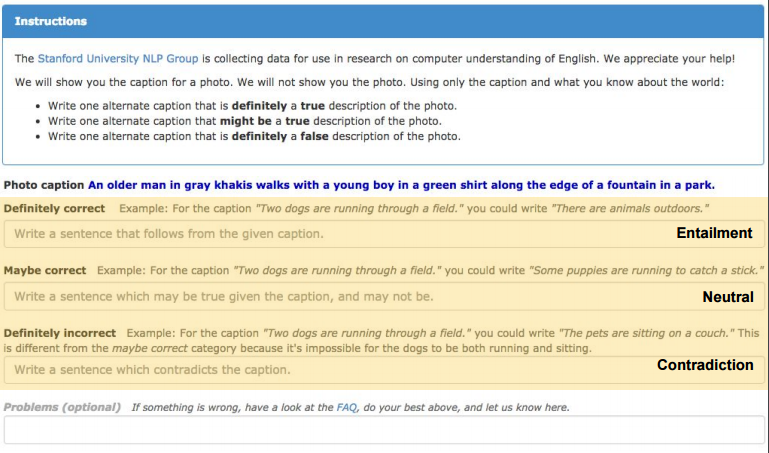
\includegraphics[scale=0.5]{data_collecting}
    \caption{Crowd-sourcing on Amazon Mechanical Turk\footnotemark}
  \end{figure}
  \footnotetext{https://www.nyu.edu/projects/bowman/cusp\_snli\_slides.pdf}
\end{frame}

\begin{frame}{SNLI Corpus}{Data collection}
  \begin{figure}[h]
    \centering
    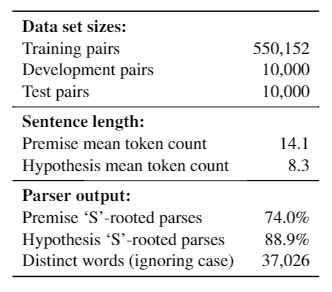
\includegraphics[scale=0.5]{data_collection}
    \caption{Key statistics for the raw sentence pairs in SNLI}
  \end{figure}
\end{frame}

\begin{frame}{SNLI Corpus}{Data validation}
  \begin{figure}[h]
    \centering
    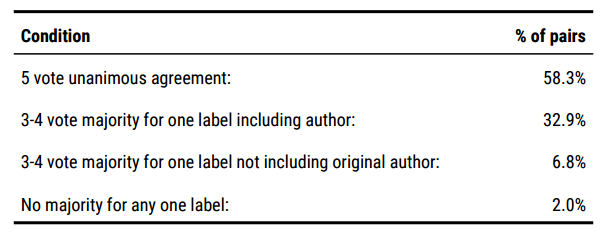
\includegraphics[scale=0.5]{data_validation}
    \caption{Data validation with 10\% held-out data\footnotemark}
  \end{figure}
  \footnotetext{https://www.nyu.edu/projects/bowman/cusp\_snli\_slides.pdf}
\end{frame}


\section{Methods}

\subsection{Feature-based}

\begin{frame}{Feature-based}{Feature selection}
  \begin{enumerate}
      \item \textbf{BLEU score} of the hypothesis with respect to the premise (n-gram =1..4)
      \item \textbf{Length difference} between the hypothesis and the premise
      \item \textbf{Count \& percentage of  overlapping words}  in  the  premise and hypothesis (all and just nouns, verbs, adjectives, and adverbs)
      \item \textbf{Unigram and bigram} in the hypothesis.
      \item \textbf{Cross-unigrams}: for  every  pair  of  words across  the  premise  and  hypothesis  which share a POS tag.
      \item \textbf{Cross-bigrams}: for  every  pair  of  bigrams across  the  premise  and  hypothesis  which share a POS tag on the second word.
  \end{enumerate}
\end{frame}

\subsection{Sentence embedding}

\begin{frame}{Sentence embedding}{Word embeddings}
    \begin{itemize}
        \item Represent words as a vectors
            \begin{itemize}
                \item $cat \Rightarrow [0.4, 0.3,..., 0.1]$
                \item $dog \Rightarrow [0.1, 0.5,..., 0.2]$
            \end{itemize}
        \item Word2vec \cite{mikolov2013distributed}
    \end{itemize}
\end{frame}

\begin{frame}{Sentence embedding}{\cite{snli:emnlp2015}}
  \begin{figure}[h]
    \centering
    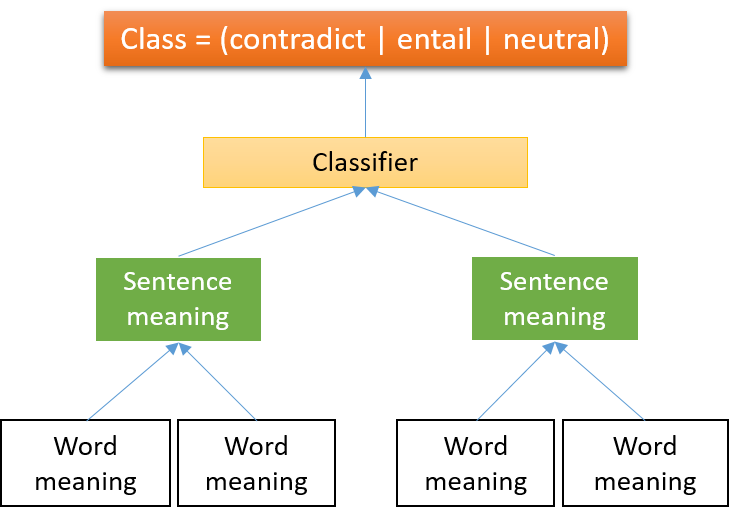
\includegraphics[scale=0.5]{neural2}
  \end{figure}
\end{frame}

\begin{frame}{Sentence embedding}{Neural network - a quick look}
    Learning a function
  \begin{figure}[h]
    \centering
    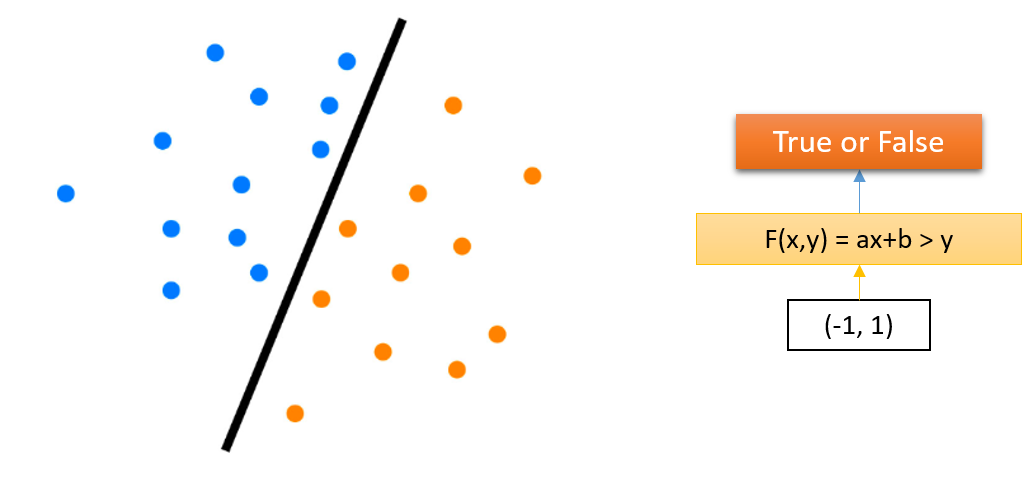
\includegraphics[scale=0.5]{neural1}
  \end{figure}
\end{frame}

\begin{frame}{Sentence embedding}{\cite{snli:emnlp2015}}
  \begin{figure}[h]
    \centering
    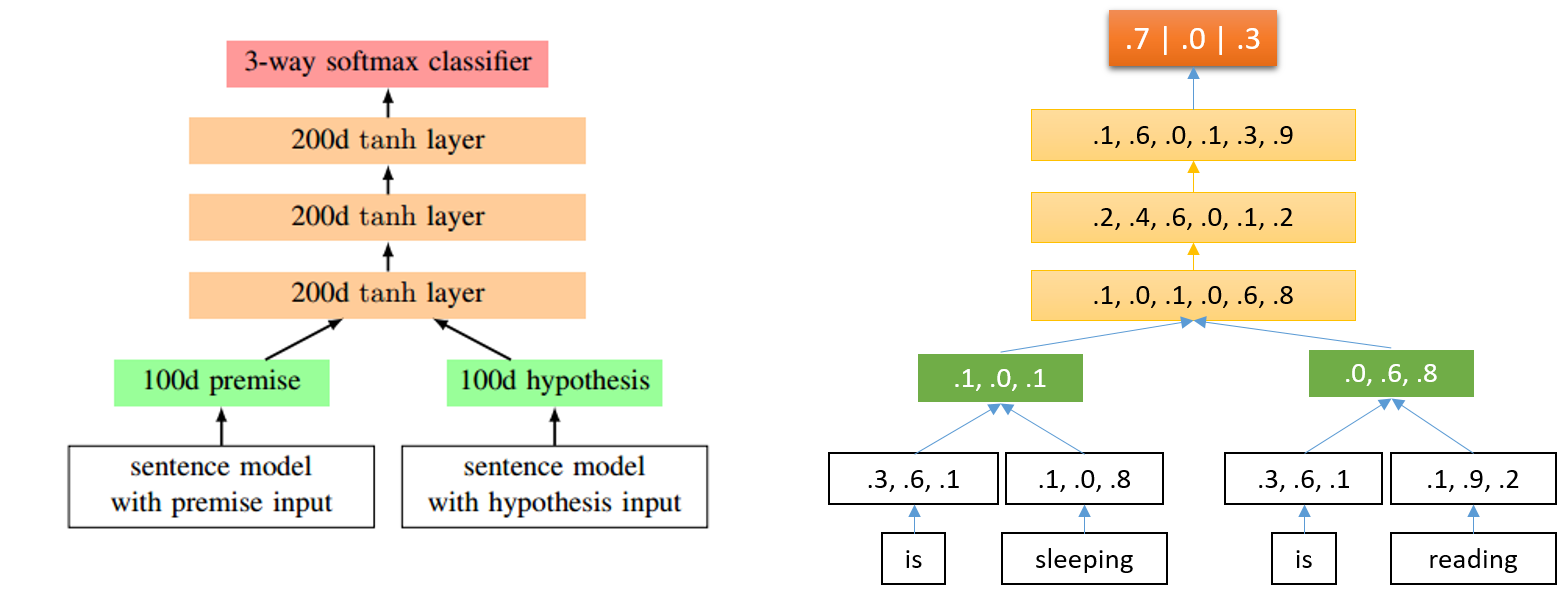
\includegraphics[scale=0.38]{sentence_encoder}
    \caption{Neural network classification architecture}
  \end{figure}
\end{frame}

\begin{frame}{Sentence embedding}{\cite{snli:emnlp2015}}
  \begin{figure}[h]
    \centering
    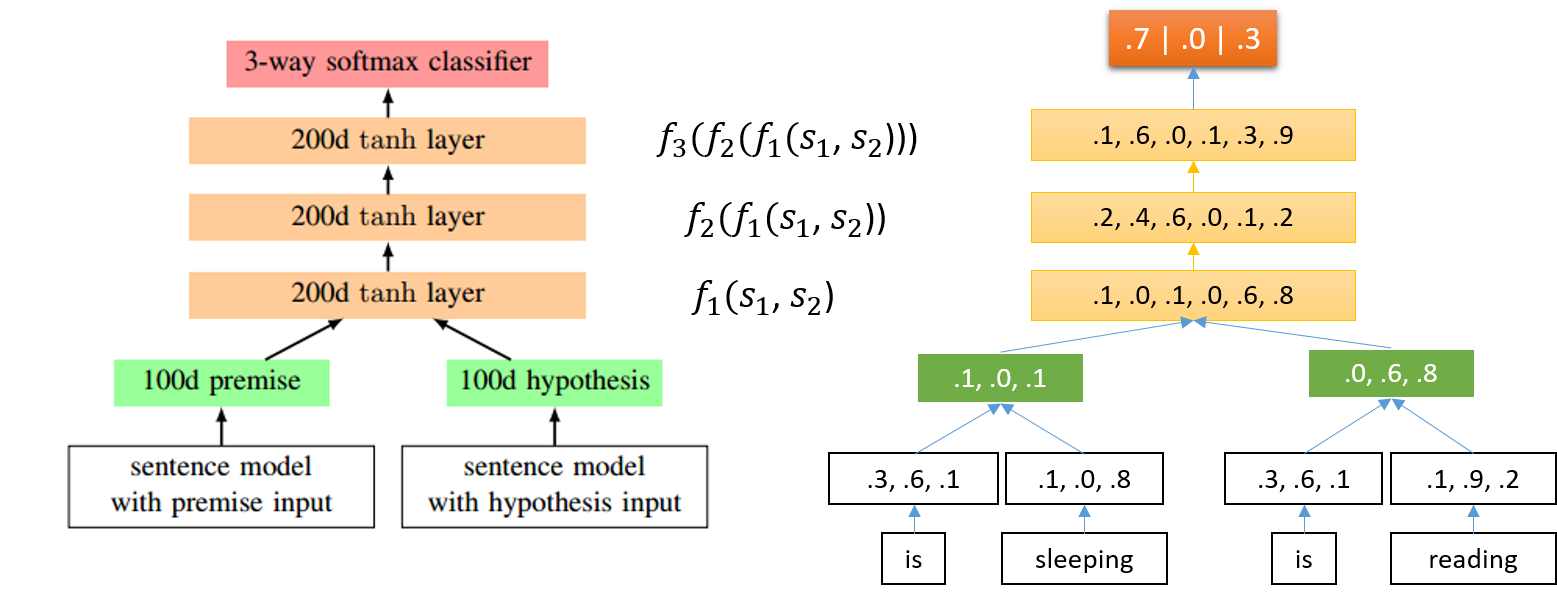
\includegraphics[scale=0.38]{sentence_encoder2}
    \caption{Neural network classification architecture}
  \end{figure}
\end{frame}

\section{Results}

\begin{frame}{Results}{Feature-based}
  \begin{figure}[h]
    \centering
    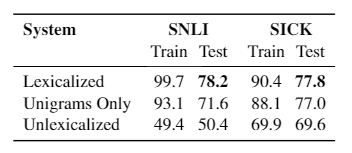
\includegraphics[scale=0.6]{nli_result3}
    \caption{Feature-based variants}
  \end{figure}
\end{frame}

\begin{frame}{Results}{Feature-based vs. Sentence embedding}
  \begin{figure}[h]
    \centering
    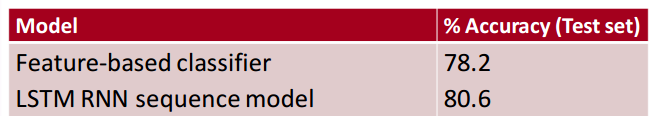
\includegraphics[scale=0.5]{nli_result2}
    \caption{Results\footnotemark}
  \end{figure}
  \footnotetext{https://nlp.stanford.edu/manning/talks/SIGIR2016-Deep-Learning-NLI.pdf}
\end{frame}

% Placing a * after \section means it will not show in the
% outline or table of contents.
\section*{Summary}

\begin{frame}{Summary}
    \begin{itemize}
        \item A large-scale, naturalistic corpus of sentence pairs labeled for entailment, contradiction, and independence.
        \item Both simple lexicalised models and neural network models perform well.
    \end{itemize}

    \begin{itemize}
        \item The RepEval 2017 Shared Task 
        \begin{itemize}
            \item https://repeval2017.github.io/shared/
        \end{itemize}
    \end{itemize}
    
\end{frame}



% All of the following is optional and typically not needed. 
\appendix
\section<presentation>*{\appendixname}
\begin{frame}[allowframebreaks]
  \frametitle<presentation>{References}
    
	\printbibliography
\end{frame}

\end{document}


